\documentclass[tikz,border=0pt]{standalone}
\usepackage[T1]{fontenc}
\usepackage{lmodern}
\usepackage{amsmath}
\usetikzlibrary{arrows.meta,positioning,fit}

\definecolor{ink}{HTML}{172033}
\definecolor{muted}{HTML}{60646B}
\definecolor{panel}{HTML}{FAFAFA}
\definecolor{rule}{HTML}{B8B8B8}

\begin{document}
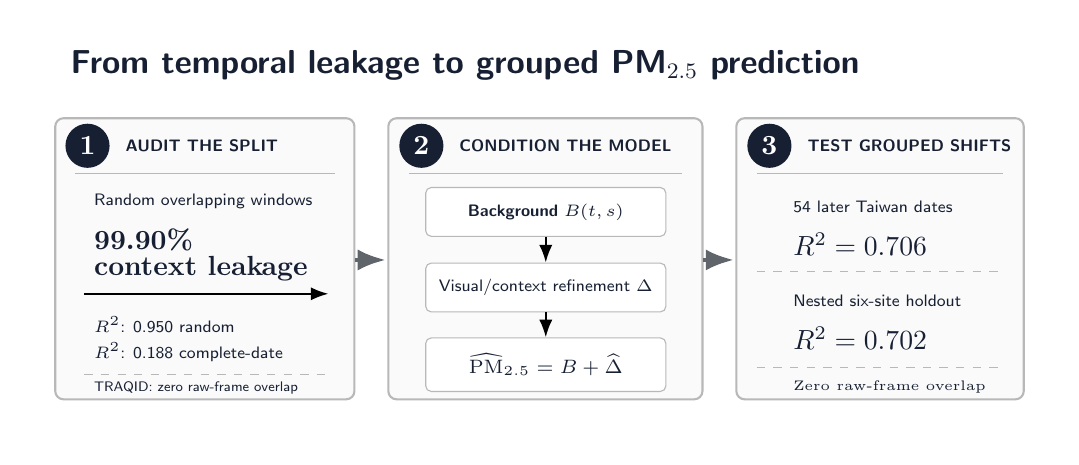
\begin{tikzpicture}[x=1cm,y=1cm,font=\sffamily\fontsize{6.3}{7.3}\selectfont,text=ink,>=Latex]
  \path[fill=white] (0,0) rectangle (13,5.2);

  \node[anchor=west,font=\sffamily\bfseries\fontsize{12}{13}\selectfont] at (0.42,4.72)
    {From temporal leakage to grouped PM$_{2.5}$ prediction};
  \draw[rounded corners=3pt,fill=panel,draw=rule,line width=0.75pt]
    (0.35,0.48) rectangle (4.15,4.05);
  \node[circle,fill=ink,text=white,inner sep=2.6pt,font=\bfseries] at (0.76,3.70) {1};
  \node[anchor=west,font=\sffamily\bfseries\fontsize{6.1}{7}\selectfont] at (1.12,3.70) {AUDIT THE SPLIT};
  \draw[rule] (0.60,3.35) -- (3.90,3.35);
  \node[anchor=west] at (0.72,3.00) {Random overlapping windows};
  \node[anchor=west,font=\bfseries\fontsize{10}{10.5}\selectfont] at (0.72,2.50) {99.90\%};
  \node[anchor=west,font=\bfseries] at (0.72,2.14) {context leakage};
  \draw[->,line width=0.75pt] (0.72,1.82) -- (3.82,1.82);
  \node[anchor=west] at (0.72,1.43) {$R^2$: 0.950 random};
  \node[anchor=west] at (0.72,1.08) {$R^2$: 0.188 complete-date};
  \draw[rule,dashed] (0.72,0.80) -- (3.82,0.80);
  \node[anchor=west,font=\sffamily\fontsize{5.0}{5.8}\selectfont] at (0.72,0.62) {TRAQID: zero raw-frame overlap};

  \draw[rounded corners=3pt,fill=panel,draw=rule,line width=0.75pt]
    (4.58,0.48) rectangle (8.57,4.05);
  \node[circle,fill=ink,text=white,inner sep=2.6pt,font=\bfseries] at (5.00,3.70) {2};
  \node[anchor=west,font=\sffamily\bfseries\fontsize{6.1}{7}\selectfont] at (5.36,3.70) {CONDITION THE MODEL};
  \draw[rule] (4.84,3.35) -- (8.31,3.35);
  \node[draw=rule,rounded corners=2pt,fill=white,minimum width=3.05cm,
        minimum height=0.62cm] (bg) at (6.58,2.86) {\textbf{Background} $B(t,s)$};
  \node[draw=rule,rounded corners=2pt,fill=white,minimum width=3.05cm,
        minimum height=0.62cm] (ref) at (6.58,1.90) {Visual/context refinement $\Delta$};
  \node[draw=rule,rounded corners=2pt,fill=white,minimum width=3.05cm,
        minimum height=0.68cm,font=\bfseries\fontsize{7.2}{8}\selectfont]
        (out) at (6.58,0.92) {$\widehat{\mathrm{PM}}_{2.5}=B+\widehat{\Delta}$};
  \draw[->,line width=0.75pt] (bg) -- (ref);
  \draw[->,line width=0.75pt] (ref) -- (out);

  \draw[rounded corners=3pt,fill=panel,draw=rule,line width=0.75pt]
    (9.00,0.48) rectangle (12.65,4.05);
  \node[circle,fill=ink,text=white,inner sep=2.6pt,font=\bfseries] at (9.42,3.70) {3};
  \node[anchor=west,font=\sffamily\bfseries\fontsize{6.1}{7}\selectfont] at (9.78,3.70) {TEST GROUPED SHIFTS};
  \draw[rule] (9.26,3.35) -- (12.39,3.35);
  \node[anchor=west] at (9.60,2.93) {54 later Taiwan dates};
  \node[anchor=west,font=\bfseries\fontsize{10}{10.5}\selectfont] at (9.60,2.45) {$R^2=0.706$};
  \draw[rule,dashed] (9.26,2.10) -- (12.39,2.10);
  \node[anchor=west] at (9.60,1.73) {Nested six-site holdout};
  \node[anchor=west,font=\bfseries\fontsize{10}{10.5}\selectfont] at (9.60,1.25) {$R^2=0.702$};
  \draw[rule,dashed] (9.26,0.88) -- (12.39,0.88);
  \node[anchor=west,font=\fontsize{5.5}{6.2}\selectfont] at (9.60,0.64) {Zero raw-frame overlap};

  \draw[->,line width=1.6pt,draw=muted] (4.16,2.25) -- (4.55,2.25);
  \draw[->,line width=1.6pt,draw=muted] (8.58,2.25) -- (8.97,2.25);
\end{tikzpicture}
\end{document}
